% Gemini theme
% https://github.com/anishathalye/gemini
%
% We try to keep this Overleaf template in sync with the canonical source on
% GitHub, but it's recommended that you obtain the template directly from
% GitHub to ensure that you are using the latest version.

\documentclass[final]{beamer}

% ====================
% Packages
% ====================

\usepackage[T1]{fontenc}
\usepackage{lmodern}
\usepackage{beamerposter}
\geometry{papersize={841mm,1188mm}}
\usetheme{gemini}
\usecolortheme{gemini}
\usepackage{graphicx}
\usepackage{booktabs}
\usepackage{tikz}
\usepackage{pgfplots}
\pgfplotsset{compat=1.14}
\renewcommand{\d}{\textrm{d}}
% ====================
% Lengths
% ====================

% If you have N columns, choose \sepwidth and \colwidth such that
% (N+1)*\sepwidth + N*\colwidth = \paperwidth
\newlength{\sepwidth}
\newlength{\colwidth}
\setlength{\sepwidth}{0.025\paperwidth}
\setlength{\colwidth}{0.3\paperwidth}

\newcommand{\separatorcolumn}{\begin{column}{\sepwidth}\end{column}}

% ====================
% Title
% ====================

\title{Ab Initio Study into the Reorientation Rates of NnVH Defects}
\title{Ab Initio Study of Hydrogen Quantum Tunnelling in NnVH Defects}


\author{Samuel J. Frost}

\institute[shortinst]{University of Warwick}

% ====================
% Footer (optional)
% ====================

\footercontent{
  \href{https://www.samuelfrost.co.uk}{https://www.samuelfrost.co.uk} \hfill
  \href{mailto:alyssa.p.hacker@example.com}{Samuel.Frost@Warwick.ac.uk}}
% (can be left out to remove footer)

% ====================
% Logo (optional)
% ====================

% use this to include logos on the left and/or right side of the header:
% \logoright{\includegraphics[height=7cm]{logo1.pdf}}
% \logoleft{\includegraphics[height=7cm]{logo2.pdf}}

% ====================
% Body
% ====================

\begin{document}

\begin{frame}[t]
\begin{columns}[t]
\separatorcolumn

\begin{column}{\colwidth}
    
  \begin{block}{NnVH Defects in Diamond}
    \begin{itemize}
        \item NnVH defects contain a central vacancy, surrounded by $n$ substitutional nitrogens, where $n \in [0, 3]$, as well as a hydrogen sitting in the vacancy.
        \item The original proposed structure of these defects were the hydrogen being bonded to one of the unsaturated carbons surrounding the vacancy, giving rise to a low order point group. (NOT REALLY)
        \item EPR experiments observe a higher order point group, leading to the suspicion that the hydrogen was bonded to one of the nitrogens, however ab initio studies show that this is too energetically unfavourable.
        \item This lead to the theory that the hydrogen is rapidly reorientating \emph{between} carbon atoms at a rate fast enough that it shows a higher order averaged symmetry when observed under EPR.
        \item Classical estimates for the reorientation give incredibly low rates for reorientation, with hydrogen staying at one carbon site for over 300s, much too slow to show averaged symmetry under EPR, which measures at rates in the GHz range. This is shown below in equation .
        \item This gave rise to the now widely accepted theory that the hydrogen is in fact \emph{quantum tunnelling} between equivalent carbon sites.
    \end{itemize}

    
    \begin{figure}
      \centering
        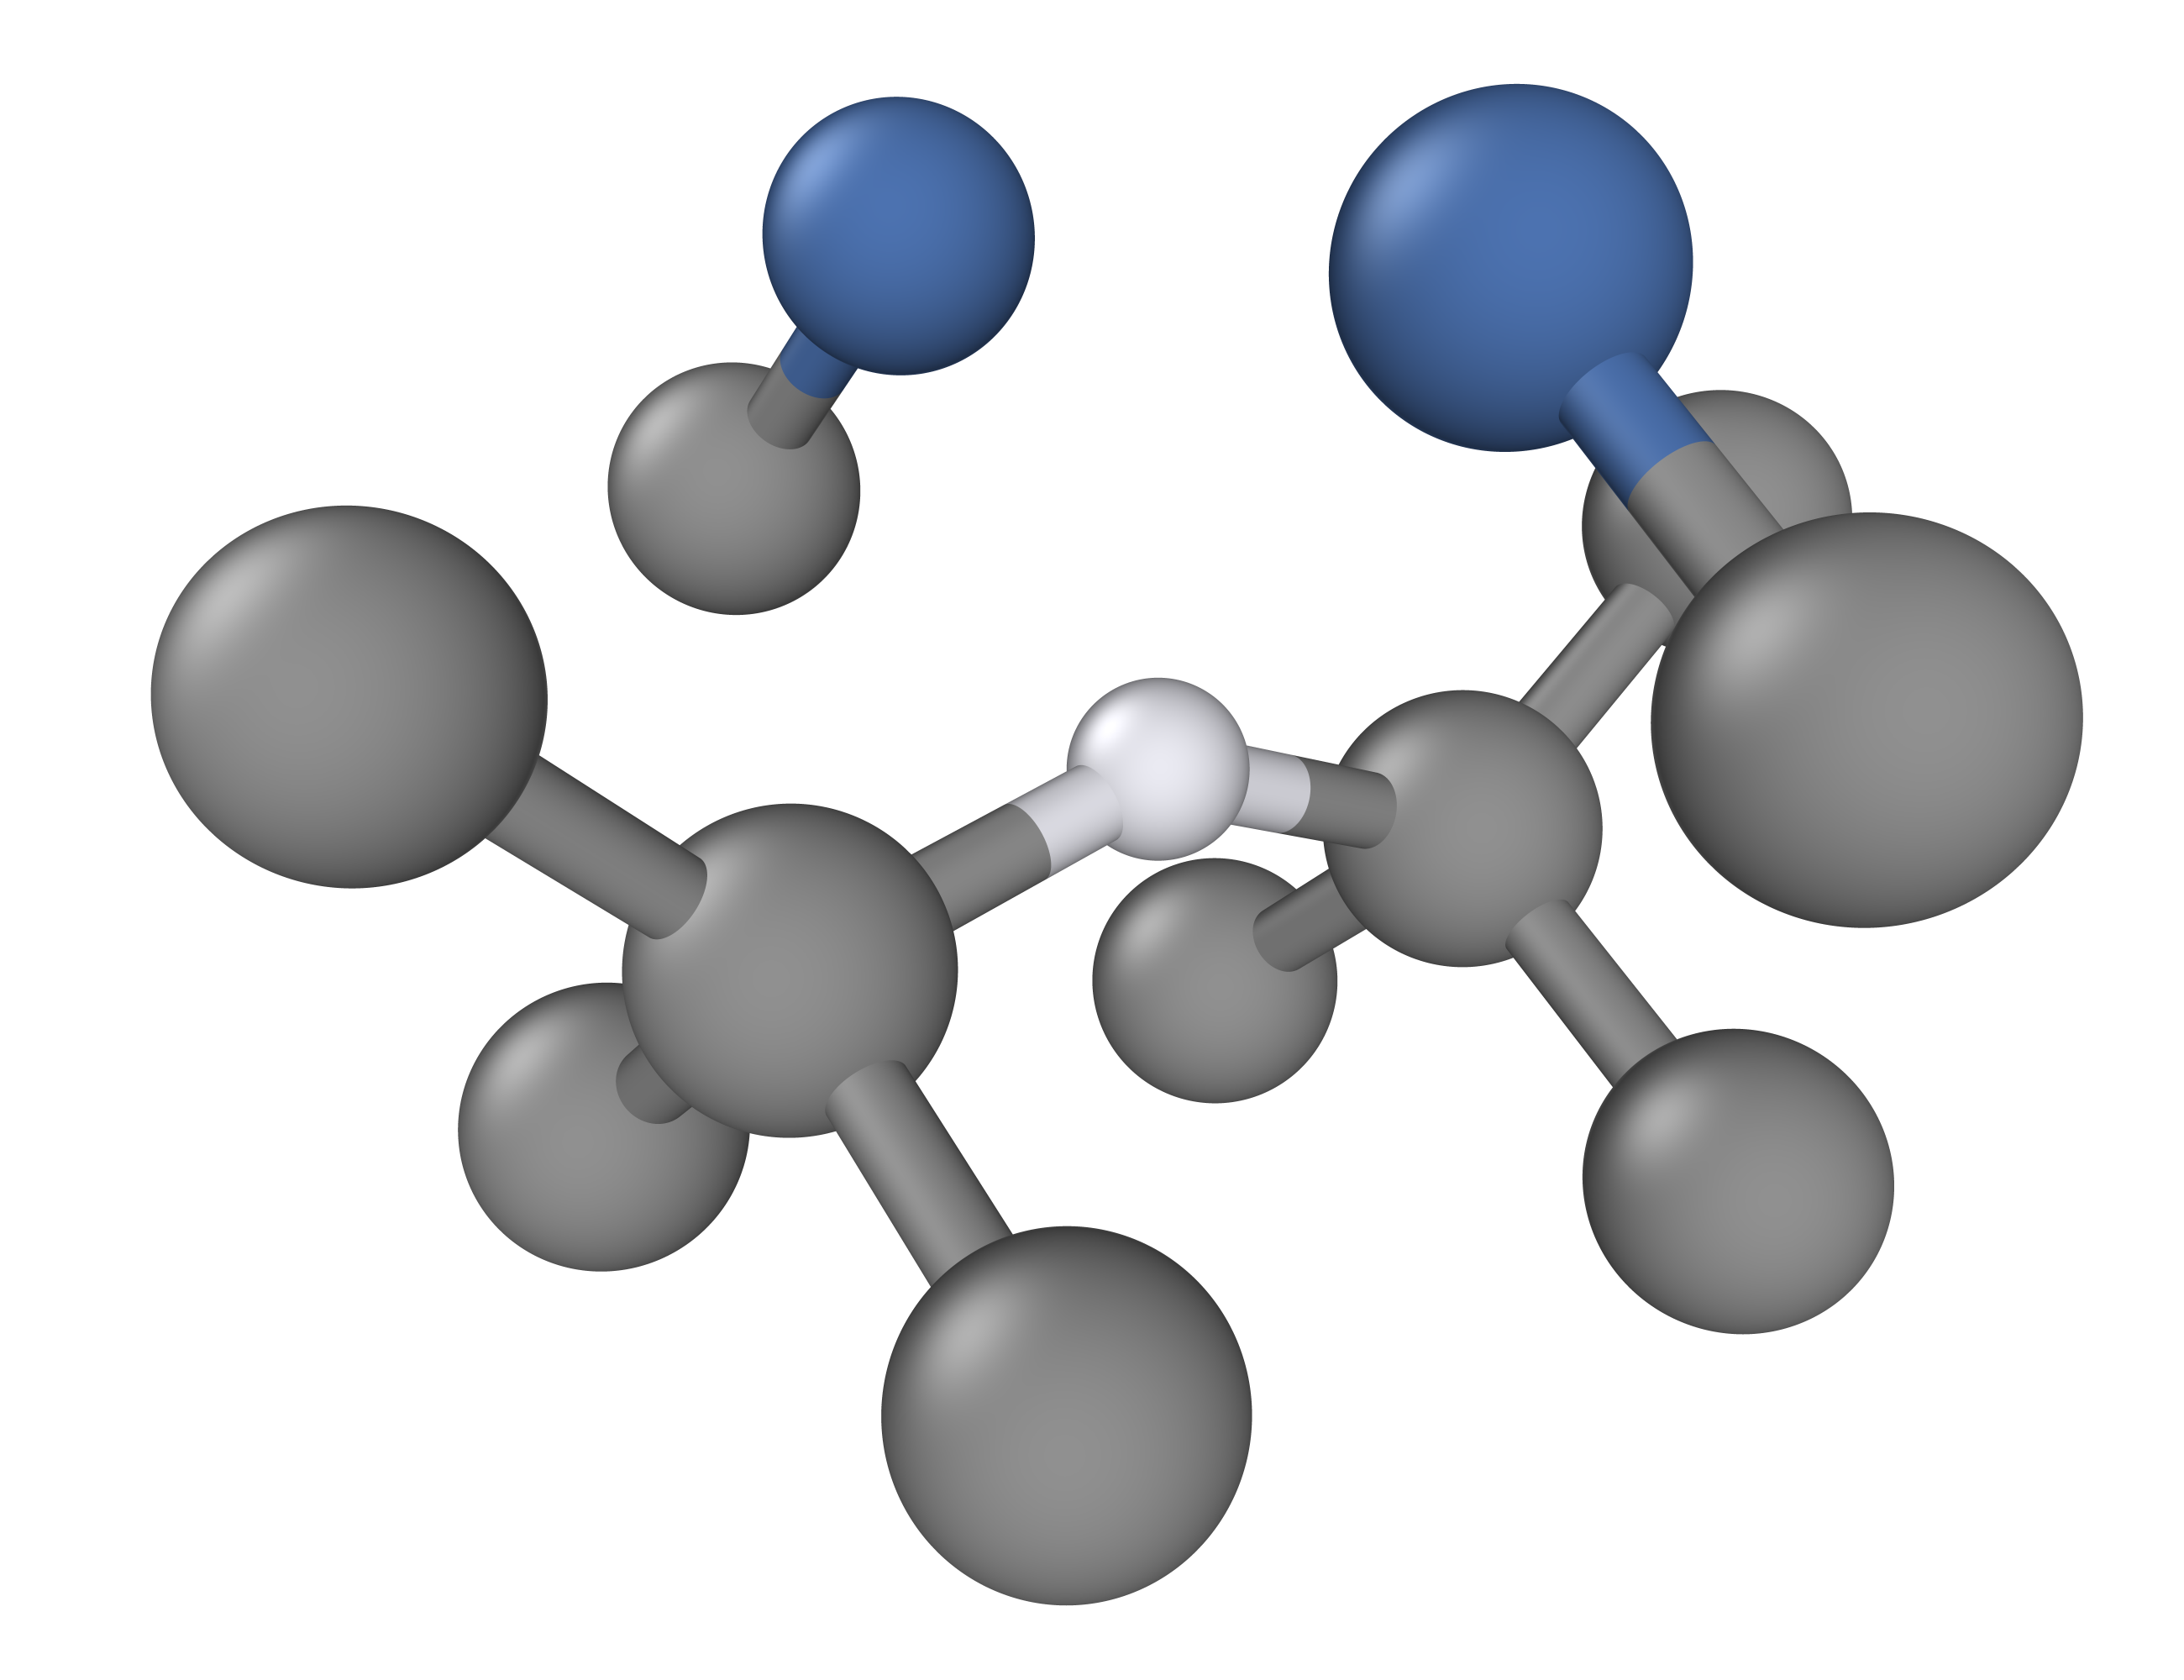
\includegraphics[width=\textwidth]{n2vh_coloured.png}
      \caption{N$_2$VH in its averaged C$_{2v}$ symmetry position, switching rapidly between the two of them. Hydrogen is shown in white, nitrogen in blue, and carbon in grey, most of the surrounding structure has been omitted for clarity. Generated using OVITO.}
    \end{figure}



  \end{block}

  \begin{block}{Attempt Frequency from Phonon Modes}
    \begin{itemize}
        \item In order to calculator the tunnelling rate, the attempt frequency over the barrier must be known.
        \item This can be approximated as the vibrational frequency of hydrogen in the \emph{direction} of the reaction coordinate, $\nu$.
        \item \textbf{Finite displacement phonon calculations} were performed to calculate the phonon modes pertaining to each atom. A $3N\times3N$ \emph{dynamical matrix} is retrieved, which contains the force acted on each atom due to the displacement of another when moved a finite displacement from its minimum energy point.
        \item This can be represented mathematically by equation , where $E$ is energy, $r_n$ is the displacement(?) of an atom and $m_n$ is its corresponding mass, where $i$ and $j$ occur for every possible pair of atoms.
    \end{itemize}
    \begin{align*}
        \frac{{\d}^2E}{{\d}r_i\,{\d}r_j}\frac{1}{\sqrt{m_i\,m_j}}
    \end{align*}
    \begin{itemize}
        \item From here we can diagonalise the matrix to retrieve its eigenvalues and eigenvectors, which detail the strength and direction of each phonon mode.
        \item The dot of product of these modes, with the normalised direction of the reaction coordinate will give the tunnelling frequency, $\nu$.
    \end{itemize}

  \end{block}

  \begin{alertblock}{Computational Details}
    \begin{itemize}
        \item All calculations were performed using CASTEP 23.1, using a periodic 64 atom simulation cell.
        \item The meta-GGA RSCAN functional was used for all calculations unless stated otherwise. 
        \item A plane wave cut-off of $1\,000$ eV and a $4\times 4\times 4$ monkhorst-pack k-point grid was used, with a force tolerance of 0.02 eV / {\AA} for geometrical minimisation.
        \item A lattice constant of 3.5537 was found during convergence testing, close to the experimental value of 3.567.
    \end{itemize}

  \end{alertblock}

\end{column}

\separatorcolumn

\begin{column}{\colwidth}

  \begin{block}{Probability of Tunnelling}
    % To study the energy barrier that is required to be overcame in order for the hydrogen to tunnel, nudged elastic band (NEB) calculations were performed. This takes the form of multiple \emph{images} between an initial and final state connected by \emph{springs}, such that an equal force is applied between each image. This ensures that during the minimisation procedure each image does not simply minimise to the lowest possible state. This finds the \emph{minimum energy path}, between the two carbons which the hydrogen is tunnelling between, giving a reaction coordinate for the quantum tunnelling. Due to the computational intensity of these calculations, only a small number of points along the reaction coordinate can be sampled, in order to fill in the gaps, Gaussian Process Regression (GPR) can be employed to interpolate the data.  

    \begin{itemize}
      \item \textbf{Nudged Elastic Band (NEB)} calculations were performed to find the energy along the reaction coordinate of the tunnelling hydrogen for each NnVH system.
      \item \textbf{Gaussian Process Regression} was employed to interpolate between the discrete points along the reaction coordinate such that continuous integration could be performed later.
      \item \textbf{The WKB approximation} was then used to calculate the instantaneous probability of tunnelling.  
    \end{itemize}
    \begin{align*}        
        P &= \exp \left(\frac{-4\pi}{h}\int_a^b \sqrt{2m\,(V-E)}  \right)
    \end{align*}
    In this equation, the integral is performed between the \emph{turning points} of the energy barrier, $a$ and $b$, where the potential and energy of the system are equal, such that $V = E$. 


  \end{block}

  \begin{block}{Fusce aliquam magna velit}

    Et rutrum ex euismod vel. Pellentesque ultricies, velit in fermentum
    vestibulum, lectus nisi pretium nibh, sit amet aliquam lectus augue vel
    velit. Suspendisse rhoncus massa porttitor augue feugiat molestie. Sed
    molestie ut orci nec malesuada. Sed ultricies feugiat est fringilla
    posuere.

    \begin{figure}
      \centering
      \begin{tikzpicture}
        \begin{axis}[
            scale only axis,
            no markers,
            domain=0:2*pi,
            samples=100,
            axis lines=center,
            axis line style={-},
            ticks=none]
          \addplot[red] {sin(deg(x))};
          \addplot[blue] {cos(deg(x))};
        \end{axis}
      \end{tikzpicture}
      \caption{Another figure caption.}
    \end{figure}

  \end{block}

  \begin{block}{Nam cursus consequat egestas}

    Nulla eget sem quam. Ut aliquam volutpat nisi vestibulum convallis. Nunc a
    lectus et eros facilisis hendrerit eu non urna. Interdum et malesuada fames
    ac ante \textit{ipsum primis} in faucibus. Etiam sit amet velit eget sem
    euismod tristique. Praesent enim erat, porta vel mattis sed, pharetra sed
    ipsum. Morbi commodo condimentum massa, \textit{tempus venenatis} massa
    hendrerit quis. Maecenas sed porta est. Praesent mollis interdum lectus,
    sit amet sollicitudin risus tincidunt non.

    Etiam sit amet tempus lorem, aliquet condimentum velit. Donec et nibh
    consequat, sagittis ex eget, dictum orci. Etiam quis semper ante. Ut eu
    mauris purus. Proin nec consectetur ligula. Mauris pretium molestie
    ullamcorper. Integer nisi neque, aliquet et odio non, sagittis porta justo.

    \begin{itemize}
      \item \textbf{Sed consequat} id ante vel efficitur. Praesent congue massa
        sed est scelerisque, elementum mollis augue iaculis.
        \begin{itemize}
          \item In sed est finibus, vulputate
            nunc gravida, pulvinar lorem. In maximus nunc dolor, sed auctor eros
            porttitor quis.
          \item Fusce ornare dignissim nisi. Nam sit amet risus vel lacus
            tempor tincidunt eu a arcu.
          \item Donec rhoncus vestibulum erat, quis aliquam leo
            gravida egestas.
        \end{itemize}
      \item \textbf{Sed luctus, elit sit amet} dictum maximus, diam dolor
        faucibus purus, sed lobortis justo erat id turpis.
      \item \textbf{Pellentesque facilisis dolor in leo} bibendum congue.
        Maecenas congue finibus justo, vitae eleifend urna facilisis at.
    \end{itemize}
    
\begin{figure}[htbp]
    \centering
    % Set the width of the figure

    \resizebox{\textwidth}{!}{
    % This file was created with tikzplotlib v0.10.1.
\begin{tikzpicture}[font=\fontsize{6}{7}\selectfont]
% This file was created with tikzplotlib v0.10.1.
\definecolor{darkslategray38}{RGB}{38,38,38}
\definecolor{lavender234234242}{RGB}{234,234,242}
\definecolor{mediumseagreen85168104}{RGB}{85,168,104}
\definecolor{steelblue76114176}{RGB}{76,114,176}

\begin{axis}[
axis background/.style={fill=lavender234234242},
axis line style={white},
legend cell align={left},
legend style={
  fill opacity=0.8,
  draw opacity=1,
  text opacity=1,
  at={(0.5,0.09)},
  anchor=south,
  draw=none,
  fill=lavender234234242
},
ylabel shift = -12 pt,
xlabel shift = -12 pt,
tick align=outside,
tick pos=left,
x grid style={white},
xlabel=\textcolor{darkslategray38}{\fontsize{8}{9}\selectfont Reaction Coordinate / {\AA} },
xmajorgrids,
xmin=-0.0540455025233226, xmax=1.13495555298978,
xtick style={color=darkslategray38},
y grid style={white},
ylabel=\textcolor{darkslategray38}{\fontsize{8}{9}\selectfont Barrier Height / eV},
ymajorgrids,
ymin=-0.0218074212401964, ymax=0.430657530668547,
ytick style={color=darkslategray38}
]
\addplot [draw=steelblue76114176, fill=steelblue76114176, mark=*, only marks]
table{%
x  y
0 0
0.145478959605773 0.0421025100004044
0.932704224327079 0.044033109999873
0.331610559783429 0.232790449999811
0.746958798653657 0.236188139999285
0.538821061179613 0.409716329999355
1.08091005046645 -1.07000050775241e-06
};
\addlegendentry{Observations}
\path [fill=mediumseagreen85168104, fill opacity=0.5, line width=0.12pt]
(axis cs:0,1.96005085623076e-05)
--(axis cs:0,-1.9599488979334e-05)
--(axis cs:0.00434100421874077,-0.000446509521810643)
--(axis cs:0.00868200843748155,-0.000785915387606347)
--(axis cs:0.0130230126562223,-0.00101844037290698)
--(axis cs:0.0173640168749631,-0.00114389750873404)
--(axis cs:0.0217050210937039,-0.00116220591547595)
--(axis cs:0.0260460253124446,-0.00107335041705555)
--(axis cs:0.0303870295311854,-0.000877374090487393)
--(axis cs:0.0347280337499262,-0.000574374902621239)
--(axis cs:0.039069037968667,-0.000164503237289819)
--(axis cs:0.0434100421874077,0.000352040318129305)
--(axis cs:0.0477510464061485,0.000975007090753515)
--(axis cs:0.0520920506248893,0.00170410239221385)
--(axis cs:0.0564330548436301,0.00253898755221495)
--(axis cs:0.0607740590623708,0.00347928191416951)
--(axis cs:0.0651150632811116,0.00452456478663674)
--(axis cs:0.0694560674998524,0.00567437734194427)
--(axis cs:0.0737970717185931,0.00692822445256135)
--(axis cs:0.0781380759373339,0.0082855764553976)
--(axis cs:0.0824790801560747,0.00974587083408931)
--(axis cs:0.0868200843748155,0.0113085138092815)
--(axis cs:0.0911610885935562,0.0129728818270778)
--(axis cs:0.095502092812297,0.0147383229355073)
--(axis cs:0.0998430970310378,0.0166041580385663)
--(axis cs:0.104184101249779,0.0185696820161187)
--(axis cs:0.108525105468519,0.0206341646950407)
--(axis cs:0.11286610968726,0.0227968516499548)
--(axis cs:0.117207113906001,0.0250569647946369)
--(axis cs:0.121548118124742,0.0274137026785673)
--(axis cs:0.125889122343482,0.0298662402620682)
--(axis cs:0.130230126562223,0.0324137274406657)
--(axis cs:0.134571130780964,0.0350552832821397)
--(axis cs:0.138912134999705,0.0377899669199299)
--(axis cs:0.143253139218446,0.0406164104541902)
--(axis cs:0.147594143437186,0.0431788839579744)
--(axis cs:0.151935147655927,0.0454669882080134)
--(axis cs:0.156276151874668,0.0478591618617882)
--(axis cs:0.160617156093409,0.0503584499496212)
--(axis cs:0.164958160312149,0.0529672361835934)
--(axis cs:0.16929916453089,0.0556876387236719)
--(axis cs:0.173640168749631,0.0585215333653126)
--(axis cs:0.177981172968372,0.061470552803083)
--(axis cs:0.182322177187112,0.0645360821225574)
--(axis cs:0.186663181405853,0.0677192536990135)
--(axis cs:0.191004185624594,0.0710209422705625)
--(axis cs:0.195345189843335,0.0744417604301025)
--(axis cs:0.199686194062076,0.077982054633349)
--(axis cs:0.204027198280816,0.081641901770147)
--(axis cs:0.208368202499557,0.0854211063263424)
--(axis cs:0.212709206718298,0.0893191981543445)
--(axis cs:0.217050210937039,0.0933354308652096)
--(axis cs:0.221391215155779,0.0974687808519841)
--(axis cs:0.22573221937452,0.101717946951117)
--(axis cs:0.230073223593261,0.106081350747001)
--(axis cs:0.234414227812002,0.110557137522385)
--(axis cs:0.238755232030743,0.11514317785559)
--(axis cs:0.243096236249483,0.119837069863636)
--(axis cs:0.247437240468224,0.124636142088548)
--(axis cs:0.251778244686965,0.129537457022196)
--(axis cs:0.256119248905706,0.134537815263355)
--(axis cs:0.260460253124446,0.139633760298756)
--(axis cs:0.264801257343187,0.144821583898125)
--(axis cs:0.269142261561928,0.150097332111341)
--(axis cs:0.273483265780669,0.155456811854102)
--(axis cs:0.27782426999941,0.16089559806623)
--(axis cs:0.28216527421815,0.166409041424873)
--(axis cs:0.286506278436891,0.171992276591942)
--(axis cs:0.290847282655632,0.177640230971523)
--(axis cs:0.295188286874373,0.18334763394712)
--(axis cs:0.299529291093113,0.189109026557125)
--(axis cs:0.303870295311854,0.194918771541777)
--(axis cs:0.308211299530595,0.200771063629753)
--(axis cs:0.312552303749336,0.206659939736555)
--(axis cs:0.316893307968076,0.212579288035158)
--(axis cs:0.321234312186817,0.218522851471875)
--(axis cs:0.325575316405558,0.224484196034405)
--(axis cs:0.329916320624299,0.230456013525651)
--(axis cs:0.33425732484304,0.236058915250833)
--(axis cs:0.33859832906178,0.241421244187183)
--(axis cs:0.342939333280521,0.246778862242976)
--(axis cs:0.347280337499262,0.252128141060039)
--(axis cs:0.351621341718003,0.25746501295747)
--(axis cs:0.355962345936743,0.262785284350401)
--(axis cs:0.360303350155484,0.268084667572434)
--(axis cs:0.364644354374225,0.273358790343849)
--(axis cs:0.368985358592966,0.27860320135042)
--(axis cs:0.373326362811707,0.283813375029352)
--(axis cs:0.377667367030447,0.288984716323074)
--(axis cs:0.382008371249188,0.294112565635384)
--(axis cs:0.386349375467929,0.299192204072676)
--(axis cs:0.39069037968667,0.304218859000841)
--(axis cs:0.39503138390541,0.309187709927352)
--(axis cs:0.399372388124151,0.314093894708821)
--(axis cs:0.403713392342892,0.318932516078733)
--(axis cs:0.408054396561633,0.323698648487131)
--(axis cs:0.412395400780374,0.328387345241884)
--(axis cs:0.416736404999114,0.332993645939154)
--(axis cs:0.421077409217855,0.33751258416916)
--(axis cs:0.425418413436596,0.341939195482084)
--(axis cs:0.429759417655337,0.346268525597608)
--(axis cs:0.434100421874077,0.350495638840248)
--(axis cs:0.438441426092818,0.354615626781701)
--(axis cs:0.442782430311559,0.358623617070122)
--(axis cs:0.4471234345303,0.362514782425426)
--(axis cs:0.45146443874904,0.366284349778585)
--(axis cs:0.455805442967781,0.369927609532103)
--(axis cs:0.460146447186522,0.373439924917846)
--(axis cs:0.464487451405263,0.376816741427869)
--(axis cs:0.468828455624004,0.380053596292895)
--(axis cs:0.473169459842744,0.38314612798249)
--(axis cs:0.477510464061485,0.38609008570054)
--(axis cs:0.481851468280226,0.388881338848561)
--(axis cs:0.486192472498967,0.391515886428965)
--(axis cs:0.490533476717707,0.393989866359318)
--(axis cs:0.494874480936448,0.396299564667056)
--(axis cs:0.499215485155189,0.398441424531484)
--(axis cs:0.50355648937393,0.400412055134292)
--(axis cs:0.507897493592671,0.402208240267356)
--(axis cs:0.512238497811411,0.403826946615952)
--(axis cs:0.516579502030152,0.405265331550027)
--(axis cs:0.520920506248893,0.40652074998571)
--(axis cs:0.525261510467634,0.407590758825736)
--(axis cs:0.529602514686374,0.408473111974758)
--(axis cs:0.533943518905115,0.409165689361792)
--(axis cs:0.538284523123856,0.409662929254693)
--(axis cs:0.542625527342597,0.409440087162348)
--(axis cs:0.546966531561337,0.408945866716042)
--(axis cs:0.551307535780078,0.408260768899654)
--(axis cs:0.555648539998819,0.407386769682174)
--(axis cs:0.55998954421756,0.406325902243668)
--(axis cs:0.564330548436301,0.405080393242434)
--(axis cs:0.568671552655041,0.403652674089885)
--(axis cs:0.573012556873782,0.402045377973639)
--(axis cs:0.577353561092523,0.400261333620702)
--(axis cs:0.581694565311264,0.398303557912093)
--(axis cs:0.586035569530004,0.396175247926362)
--(axis cs:0.590376573748745,0.393879772619167)
--(axis cs:0.594717577967486,0.391420664233704)
--(axis cs:0.599058582186227,0.388801609498371)
--(axis cs:0.603399586404967,0.386026440652073)
--(axis cs:0.607740590623708,0.383099126331134)
--(axis cs:0.612081594842449,0.380023762348834)
--(axis cs:0.61642259906119,0.376804562396335)
--(axis cs:0.620763603279931,0.373445848693252)
--(axis cs:0.625104607498671,0.369952042615097)
--(axis cs:0.629445611717412,0.366327655324227)
--(axis cs:0.633786615936153,0.362577278430294)
--(axis cs:0.638127620154894,0.358705574705654)
--(axis cs:0.642468624373635,0.354717268880342)
--(axis cs:0.646809628592375,0.35061713854055)
--(axis cs:0.651150632811116,0.346410005153829)
--(axis cs:0.655491637029857,0.342100725243231)
--(axis cs:0.659832641248598,0.337694181731771)
--(axis cs:0.664173645467338,0.333195275477558)
--(axis cs:0.668514649686079,0.328608917018994)
--(axis cs:0.67285565390482,0.323940018548239)
--(axis cs:0.677196658123561,0.319193486129952)
--(axis cs:0.681537662342302,0.314374212181233)
--(axis cs:0.685878666561042,0.309487068227205)
--(axis cs:0.690219670779783,0.304536897945327)
--(axis cs:0.694560674998524,0.299528510509791)
--(axis cs:0.698901679217265,0.294466674245513)
--(axis cs:0.703242683436005,0.289356110598347)
--(axis cs:0.707583687654746,0.284201488424562)
--(axis cs:0.711924691873487,0.27900741859503)
--(axis cs:0.716265696092228,0.273778448895996)
--(axis cs:0.720606700310968,0.268519059174364)
--(axis cs:0.724947704529709,0.263233656585399)
--(axis cs:0.72928870874845,0.257926570513716)
--(axis cs:0.733629712967191,0.252602045613957)
--(axis cs:0.737970717185932,0.247264225417188)
--(axis cs:0.742311721404672,0.241917062644108)
--(axis cs:0.746652725623413,0.236558098560646)
--(axis cs:0.750993729842154,0.230635290267408)
--(axis cs:0.755334734060895,0.224667669821254)
--(axis cs:0.759675738279635,0.218711801656941)
--(axis cs:0.764016742498376,0.21277432264597)
--(axis cs:0.768357746717117,0.206861612973364)
--(axis cs:0.772698750935858,0.200979906398513)
--(axis cs:0.777039755154598,0.19513529470141)
--(axis cs:0.781380759373339,0.189333719983894)
--(axis cs:0.78572176359208,0.183580964629206)
--(axis cs:0.790062767810821,0.177882640849771)
--(axis cs:0.794403772029562,0.172244180359554)
--(axis cs:0.798744776248302,0.166670824364984)
--(axis cs:0.803085780467043,0.161167613963186)
--(axis cs:0.807426784685784,0.155739380998197)
--(axis cs:0.811767788904525,0.150390739409836)
--(axis cs:0.816108793123265,0.145126077102089)
--(axis cs:0.820449797342006,0.139949548353503)
--(axis cs:0.824790801560747,0.134865066789003)
--(axis cs:0.829131805779488,0.129876298930119)
--(axis cs:0.833472809998228,0.124986658338709)
--(axis cs:0.837813814216969,0.120199300367103)
--(axis cs:0.84215481843571,0.115517117526177)
--(axis cs:0.846495822654451,0.110942735480427)
--(axis cs:0.850836826873192,0.106478509678008)
--(axis cs:0.855177831091932,0.102126522621313)
--(axis cs:0.859518835310673,0.0978885817821217)
--(axis cs:0.863859839529414,0.0937662181636244)
--(axis cs:0.868200843748155,0.0897606855094136)
--(axis cs:0.872541847966895,0.0858729601581092)
--(axis cs:0.876882852185636,0.0821037415398394)
--(axis cs:0.881223856404377,0.0784534533091876)
--(axis cs:0.885564860623118,0.0749222451063229)
--(axis cs:0.889905864841859,0.0715099949356462)
--(axis cs:0.894246869060599,0.0682163121464442)
--(axis cs:0.89858787327934,0.0650405409932096)
--(axis cs:0.902928877498081,0.0619817647387821)
--(axis cs:0.907269881716822,0.0590388102290128)
--(axis cs:0.911610885935562,0.0562102527725016)
--(axis cs:0.915951890154303,0.0534944208465179)
--(axis cs:0.920292894373044,0.0508893988552931)
--(axis cs:0.924633898591785,0.0483930186223193)
--(axis cs:0.928974902810526,0.0460027439138837)
--(axis cs:0.933315907029266,0.043608453387361)
--(axis cs:0.937656911248007,0.0406749363327815)
--(axis cs:0.941997915466748,0.0378303776123113)
--(axis cs:0.946338919685489,0.0350785140698837)
--(axis cs:0.950679923904229,0.0324204141449811)
--(axis cs:0.95502092812297,0.0298570469709652)
--(axis cs:0.959361932341711,0.0273893439877725)
--(axis cs:0.963702936560452,0.0250182087080268)
--(axis cs:0.968043940779193,0.0227445190680872)
--(axis cs:0.972384944997933,0.0205691279201557)
--(axis cs:0.976725949216674,0.0184928628425533)
--(axis cs:0.981066953435415,0.0165165256038616)
--(axis cs:0.985407957654156,0.0146408913989941)
--(axis cs:0.989748961872896,0.0128667079074392)
--(axis cs:0.994089966091637,0.0111946941998168)
--(axis cs:0.998430970310378,0.00962553950868976)
--(axis cs:1.00277197452912,0.00815990187633561)
--(axis cs:1.00711297874786,0.00679840668990422)
--(axis cs:1.0114539829666,0.00554164511423822)
--(axis cs:1.01579498718534,0.00439017243211518)
--(axis cs:1.02013599140408,0.00334450630186549)
--(axis cs:1.02447699562282,0.00240512494226004)
--(axis cs:1.02881799984156,0.00157246525460126)
--(axis cs:1.0331590040603,0.000846920892007387)
--(axis cs:1.03750000827904,0.000228840285128085)
--(axis cs:1.04184101249779,-0.000281475366862715)
--(axis cs:1.04618201671653,-0.000683774133736777)
--(axis cs:1.05052302093527,-0.000977855418529266)
--(axis cs:1.05486402515401,-0.00116357205972056)
--(axis cs:1.05920502937275,-0.00124083251707174)
--(axis cs:1.06354603359149,-0.00120960330057425)
--(axis cs:1.06788703781023,-0.00106991225560307)
--(axis cs:1.07222804202897,-0.000821855811811426)
--(axis cs:1.07656904624771,-0.000465638238642895)
--(axis cs:1.08091005046645,-2.06695279067983e-05)
--(axis cs:1.08091005046645,1.85304709948666e-05)
--(axis cs:1.08091005046645,1.85304709948666e-05)
--(axis cs:1.07656904624771,0.00117074655206963)
--(axis cs:1.07222804202897,0.00230287555805602)
--(axis cs:1.06788703781023,0.00339946136755978)
--(axis cs:1.06354603359149,0.00446432042962338)
--(axis cs:1.05920502937275,0.00550143817100123)
--(axis cs:1.05486402515401,0.00651492369655165)
--(axis cs:1.05052302093527,0.00750899616676262)
--(axis cs:1.04618201671653,0.00848797481500264)
--(axis cs:1.04184101249779,0.00945626950341403)
--(axis cs:1.03750000827904,0.0104183712118359)
--(axis cs:1.0331590040603,0.0113788423087737)
--(axis cs:1.02881799984156,0.0123423065681392)
--(axis cs:1.02447699562282,0.0133134389312613)
--(axis cs:1.02013599140408,0.0142969550273224)
--(axis cs:1.01579498718534,0.0152976004710281)
--(axis cs:1.0114539829666,0.0163201399598967)
--(axis cs:1.00711297874786,0.0173693461949463)
--(axis cs:1.00277197452912,0.0184499886502624)
--(axis cs:0.998430970310378,0.0195668222178396)
--(axis cs:0.994089966091637,0.020724575754974)
--(axis cs:0.989748961872896,0.0219279405624412)
--(axis cs:0.985407957654156,0.0231815588223849)
--(axis cs:0.981066953435415,0.0244900120261859)
--(axis cs:0.976725949216674,0.0258578094235553)
--(axis cs:0.972384944997933,0.0272893765271196)
--(axis cs:0.968043940779193,0.0287890437107531)
--(axis cs:0.963702936560452,0.0303610349507694)
--(axis cs:0.959361932341711,0.0320094567838328)
--(axis cs:0.95502092812297,0.0337382876238519)
--(axis cs:0.950679923904229,0.0355513677982731)
--(axis cs:0.946338919685489,0.0374523915060811)
--(axis cs:0.941997915466748,0.0394449062792409)
--(axis cs:0.937656911248007,0.0415323644050597)
--(axis cs:0.933315907029266,0.043720681974771)
--(axis cs:0.928974902810526,0.046640008614635)
--(axis cs:0.924633898591785,0.0497568742065728)
--(axis cs:0.920292894373044,0.0529626643590504)
--(axis cs:0.915951890154303,0.0562561069271828)
--(axis cs:0.911610885935562,0.0596360460133541)
--(axis cs:0.907269881716822,0.0631013178434223)
--(axis cs:0.902928877498081,0.0666507339383412)
--(axis cs:0.89858787327934,0.0702830759044982)
--(axis cs:0.894246869060599,0.0739970925500757)
--(axis cs:0.889905864841859,0.0777914975788827)
--(axis cs:0.885564860623118,0.0816649674075173)
--(axis cs:0.881223856404377,0.0856161389635489)
--(axis cs:0.876882852185636,0.0896436074169243)
--(axis cs:0.872541847966895,0.0937459238304982)
--(axis cs:0.868200843748155,0.0979215927292782)
--(axis cs:0.863859839529414,0.102169069593933)
--(axis cs:0.859518835310673,0.106486758287968)
--(axis cs:0.855177831091932,0.110873008429352)
--(axis cs:0.850836826873192,0.115326112719163)
--(axis cs:0.846495822654451,0.119844304240252)
--(axis cs:0.84215481843571,0.124425753740156)
--(axis cs:0.837813814216969,0.129068566912622)
--(axis cs:0.833472809998228,0.133770781692944)
--(axis cs:0.829131805779488,0.13853036558267)
--(axis cs:0.824790801560747,0.143345213019271)
--(axis cs:0.820449797342006,0.148213142807294)
--(axis cs:0.816108793123265,0.153131895627027)
--(axis cs:0.811767788904525,0.158099131637573)
--(axis cs:0.807426784685784,0.163112428191002)
--(axis cs:0.803085780467043,0.168169277674724)
--(axis cs:0.798744776248302,0.173267085499467)
--(axis cs:0.794403772029562,0.178403168250896)
--(axis cs:0.790062767810821,0.183574752024294)
--(axis cs:0.78572176359208,0.188778970964298)
--(axis cs:0.781380759373339,0.194012866037731)
--(axis cs:0.777039755154598,0.199273384081821)
--(axis cs:0.772698750935858,0.204557377206336)
--(axis cs:0.768357746717117,0.20986160273172)
--(axis cs:0.764016742498376,0.215182724185818)
--(axis cs:0.759675738279635,0.220517315273668)
--(axis cs:0.755334734060895,0.22586187660648)
--(axis cs:0.750993729842154,0.231212958840487)
--(axis cs:0.746652725623413,0.236616847006479)
--(axis cs:0.742311721404672,0.242582114573904)
--(axis cs:0.737970717185932,0.248546095406482)
--(axis cs:0.733629712967191,0.254495557921137)
--(axis cs:0.72928870874845,0.260423547891285)
--(axis cs:0.724947704529709,0.266323183764512)
--(axis cs:0.720606700310968,0.27218758335638)
--(axis cs:0.716265696092228,0.278009864224953)
--(axis cs:0.711924691873487,0.283783153834879)
--(axis cs:0.707583687654746,0.289500601923617)
--(axis cs:0.703242683436005,0.295155393481672)
--(axis cs:0.698901679217265,0.300740761882159)
--(axis cs:0.694560674998524,0.306250001981102)
--(axis cs:0.690219670779783,0.311676483099043)
--(axis cs:0.685878666561042,0.317013661827752)
--(axis cs:0.681537662342302,0.322255094618716)
--(axis cs:0.677196658123561,0.327394450117113)
--(axis cs:0.67285565390482,0.332425521208102)
--(axis cs:0.668514649686079,0.337342236744789)
--(axis cs:0.664173645467338,0.342138672928781)
--(axis cs:0.659832641248598,0.346809064315834)
--(axis cs:0.655491637029857,0.351347814420403)
--(axis cs:0.651150632811116,0.355749505894426)
--(axis cs:0.646809628592375,0.360008910256917)
--(axis cs:0.642468624373635,0.364120997152419)
--(axis cs:0.638127620154894,0.368080943117921)
--(axis cs:0.633786615936153,0.37188413983927)
--(axis cs:0.629445611717412,0.37552620187976)
--(axis cs:0.625104607498671,0.37900297386505)
--(axis cs:0.620763603279931,0.38231053711043)
--(axis cs:0.61642259906119,0.385445215677989)
--(axis cs:0.612081594842449,0.388403581852985)
--(axis cs:0.607740590623708,0.391182461030573)
--(axis cs:0.603399586404967,0.393778936005863)
--(axis cs:0.599058582186227,0.396190350662095)
--(axis cs:0.594717577967486,0.398414313053781)
--(axis cs:0.590376573748745,0.400448697884038)
--(axis cs:0.586035569530004,0.40229164837748)
--(axis cs:0.581694565311264,0.403941577553799)
--(axis cs:0.577353561092523,0.405397168911865)
--(axis cs:0.573012556873782,0.406657376542332)
--(axis cs:0.568671552655041,0.40772142470452)
--(axis cs:0.564330548436301,0.408588806943639)
--(axis cs:0.55998954421756,0.409259284938693)
--(axis cs:0.555648539998819,0.409732887643684)
--(axis cs:0.551307535780078,0.410009912820621)
--(axis cs:0.546966531561337,0.410090941945422)
--(axis cs:0.542625527342597,0.4099769792185)
--(axis cs:0.538284523123856,0.409748035639934)
--(axis cs:0.533943518905115,0.409852807592519)
--(axis cs:0.529602514686374,0.409767026121407)
--(axis cs:0.525261510467634,0.409486086963702)
--(axis cs:0.520920506248893,0.409009307699526)
--(axis cs:0.516579502030152,0.408336357420114)
--(axis cs:0.512238497811411,0.407467182214818)
--(axis cs:0.507897493592671,0.406401995770221)
--(axis cs:0.50355648937393,0.40514127852397)
--(axis cs:0.499215485155189,0.403685778381791)
--(axis cs:0.494874480936448,0.402036511520787)
--(axis cs:0.490533476717707,0.40019476285767)
--(axis cs:0.486192472498967,0.398162086032949)
--(axis cs:0.481851468280226,0.395940302849463)
--(axis cs:0.477510464061485,0.393531502136119)
--(axis cs:0.473169459842744,0.390938038021945)
--(axis cs:0.468828455624004,0.388162527612809)
--(axis cs:0.464487451405263,0.385207848067474)
--(axis cs:0.460146447186522,0.382077133072766)
--(axis cs:0.455805442967781,0.378773768720157)
--(axis cs:0.45146443874904,0.375301388787922)
--(axis cs:0.4471234345303,0.371663869435353)
--(axis cs:0.442782430311559,0.367865323317185)
--(axis cs:0.438441426092818,0.363910093128115)
--(axis cs:0.434100421874077,0.359802744589302)
--(axis cs:0.429759417655337,0.355548058890185)
--(axis cs:0.425418413436596,0.351151024600778)
--(axis cs:0.421077409217855,0.346616829071141)
--(axis cs:0.416736404999114,0.341950849336406)
--(axis cs:0.412395400780374,0.337158642547109)
--(axis cs:0.408054396561633,0.332245935946264)
--(axis cs:0.403713392342892,0.327218616415848)
--(axis cs:0.399372388124151,0.32208271961691)
--(axis cs:0.39503138390541,0.316844418748872)
--(axis cs:0.39069037968667,0.311510012954936)
--(axis cs:0.386349375467929,0.306085915401761)
--(axis cs:0.382008371249188,0.30057864106345)
--(axis cs:0.377667367030447,0.294994794241631)
--(axis cs:0.373326362811707,0.289341055855931)
--(axis cs:0.368985358592966,0.283624170544149)
--(axis cs:0.364644354374225,0.277850933620037)
--(axis cs:0.360303350155484,0.272028177956943)
--(axis cs:0.355962345936743,0.266162760916841)
--(axis cs:0.351621341718003,0.260261551595168)
--(axis cs:0.347280337499262,0.254331419177079)
--(axis cs:0.342939333280521,0.24837922553545)
--(axis cs:0.33859832906178,0.242411840568087)
--(axis cs:0.33425732484304,0.236436439547645)
--(axis cs:0.329916320624299,0.230699538442958)
--(axis cs:0.325575316405558,0.225339969574329)
--(axis cs:0.321234312186817,0.219988654227756)
--(axis cs:0.316893307968076,0.214648400708018)
--(axis cs:0.312552303749336,0.209322684461575)
--(axis cs:0.308211299530595,0.204014937861208)
--(axis cs:0.303870295311854,0.19872850608088)
--(axis cs:0.299529291093113,0.193466638833734)
--(axis cs:0.295188286874373,0.188232488297775)
--(axis cs:0.290847282655632,0.183029108818061)
--(axis cs:0.286506278436891,0.177859457359989)
--(axis cs:0.28216527421815,0.172726394398149)
--(axis cs:0.27782426999941,0.167632685119465)
--(axis cs:0.273483265780669,0.162581000882657)
--(axis cs:0.269142261561928,0.157573920899351)
--(axis cs:0.264801257343187,0.152613934111949)
--(axis cs:0.260460253124446,0.147703441247353)
--(axis cs:0.256119248905706,0.142844757027576)
--(axis cs:0.251778244686965,0.138040112519388)
--(axis cs:0.247437240468224,0.133291657605334)
--(axis cs:0.243096236249483,0.128601463559)
--(axis cs:0.238755232030743,0.123971525707536)
--(axis cs:0.234414227812002,0.119403766164613)
--(axis cs:0.230073223593261,0.1149000366173)
--(axis cs:0.22573221937452,0.110462121150586)
--(axis cs:0.221391215155779,0.106091739093606)
--(axis cs:0.217050210937039,0.101790547871991)
--(axis cs:0.212709206718298,0.0975601458512955)
--(axis cs:0.208368202499557,0.0934020751569348)
--(axis cs:0.204027198280816,0.0893178244566398)
--(axis cs:0.199686194062076,0.0853088316925292)
--(axis cs:0.195345189843335,0.0813764867505686)
--(axis cs:0.191004185624594,0.0775221340570169)
--(axis cs:0.186663181405853,0.0737470750936124)
--(axis cs:0.182322177187112,0.0700525708275911)
--(axis cs:0.177981172968372,0.0664398440609923)
--(axis cs:0.173640168749631,0.0629100817228184)
--(axis cs:0.16929916453089,0.0594644371770191)
--(axis cs:0.164958160312149,0.0561040327657826)
--(axis cs:0.160617156093409,0.0528299633303127)
--(axis cs:0.156276151874668,0.0496433038617482)
--(axis cs:0.151935147655927,0.0465451414081808)
--(axis cs:0.147594143437186,0.0435369798657609)
--(axis cs:0.143253139218446,0.0409954815913579)
--(axis cs:0.138912134999705,0.0389082454502136)
--(axis cs:0.134571130780964,0.0369173237733807)
--(axis cs:0.130230126562223,0.0350189250666562)
--(axis cs:0.125889122343482,0.0332094891657693)
--(axis cs:0.121548118124742,0.0314853304304908)
--(axis cs:0.117207113906001,0.0298426190485532)
--(axis cs:0.11286610968726,0.0282773857743808)
--(axis cs:0.108525105468519,0.0267855310203227)
--(axis cs:0.104184101249779,0.025362835238315)
--(axis cs:0.0998430970310378,0.02400496983751)
--(axis cs:0.095502092812297,0.0227075083867643)
--(axis cs:0.0911610885935562,0.0214659379924676)
--(axis cs:0.0868200843748155,0.020275670789461)
--(axis cs:0.0824790801560747,0.0191320555007053)
--(axis cs:0.0781380759373339,0.0180303890291599)
--(axis cs:0.0737970717185931,0.0169659280489788)
--(axis cs:0.0694560674998524,0.0159339005652253)
--(axis cs:0.0651150632811116,0.0149295174124537)
--(axis cs:0.0607740590623708,0.0139479836636714)
--(axis cs:0.0564330548436301,0.0129845099220117)
--(axis cs:0.0520920506248893,0.0120343234683554)
--(axis cs:0.0477510464061485,0.0110926792392901)
--(axis cs:0.0434100421874077,0.0101548706111114)
--(axis cs:0.039069037968667,0.00921623996742042)
--(axis cs:0.0347280337499262,0.00827218903120852)
--(axis cs:0.0303870295311854,0.00731818894816373)
--(axis cs:0.0260460253124446,0.0063497901219823)
--(axis cs:0.0217050210937039,0.00536263183931091)
--(axis cs:0.0173640168749631,0.00435245183964077)
--(axis cs:0.0130230126562223,0.00331509645345428)
--(axis cs:0.00868200843748155,0.00224653449875049)
--(axis cs:0.00434100421874077,0.00114290377854194)
--(axis cs:0,1.96005085623076e-05)
--cycle;
\addlegendimage{area legend, fill=mediumseagreen85168104, fill opacity=0.5, line width=0.12pt}
\addlegendentry{95$\%$ confidence interval}

\addplot [line width=0.7pt, steelblue76114176]
table {%
0 5.09791486802413e-10
0.00434100421874077 0.000348197128365646
0.00868200843748155 0.000730309555572073
0.0130230126562223 0.00114832804027365
0.0173640168749631 0.00160427716545336
0.0217050210937039 0.00210021296191748
0.0260460253124446 0.00263821985246337
0.0303870295311854 0.00322040742883817
0.0347280337499262 0.00384890706429364
0.039069037968667 0.0045258683650653
0.0434100421874077 0.00525345546462036
0.0477510464061485 0.00603384316502181
0.0520920506248893 0.00686921293028464
0.0564330548436301 0.00776174873711333
0.0607740590623708 0.00871363278892046
0.0651150632811116 0.0097270410995452
0.0694560674998524 0.0108041389535848
0.0737970717185931 0.0119470762507701
0.0781380759373339 0.0131579827422788
0.0824790801560747 0.0144389631673973
0.0868200843748155 0.0157920922993712
0.0911610885935562 0.0172194099097727
0.095502092812297 0.0187229156611358
0.0998430970310378 0.0203045639380381
0.104184101249779 0.0219662586272169
0.108525105468519 0.0237098478576817
0.11286610968726 0.0255371187121678
0.117207113906001 0.027449791921595
0.121548118124742 0.029449516554529
0.125889122343482 0.0315378647139188
0.130230126562223 0.0337163262536609
0.134571130780964 0.0359863035277602
0.138912134999705 0.0383491061850718
0.143253139218446 0.0408059460227741
0.147594143437186 0.0433579319118677
0.151935147655927 0.0460060648080971
0.156276151874668 0.0487512328617682
0.160617156093409 0.0515942066399669
0.164958160312149 0.054535634474688
0.16929916453089 0.0575760379503455
0.173640168749631 0.0607158075440655
0.177981172968372 0.0639551984320377
0.182322177187112 0.0672943264750743
0.186663181405853 0.0707331643963129
0.191004185624594 0.0742715381637897
0.195345189843335 0.0779091235903355
0.199686194062076 0.0816454431629391
0.204027198280816 0.0854798631133934
0.208368202499557 0.0894115907416386
0.212709206718298 0.09343967200282
0.217050210937039 0.0975629893686004
0.221391215155779 0.101780259972795
0.22573221937452 0.106090034050851
0.230073223593261 0.11049069368215
0.234414227812002 0.114980451843499
0.238755232030743 0.119557351781563
0.243096236249483 0.124219266711318
0.247437240468224 0.128963899846941
0.251778244686965 0.133788784770792
0.256119248905706 0.138691286145465
0.260460253124446 0.143668600773055
0.264801257343187 0.148717759005037
0.269142261561928 0.153835626505346
0.273483265780669 0.15901890636838
0.27782426999941 0.164264141592848
0.28216527421815 0.169567717911511
0.286506278436891 0.174925866975965
0.290847282655632 0.180334669894792
0.295188286874373 0.185790061122447
0.299529291093113 0.191287832695429
0.303870295311854 0.196823638811329
0.308211299530595 0.20239300074548
0.312552303749336 0.207991312099065
0.316893307968076 0.213613844371588
0.321234312186817 0.219255752849816
0.325575316405558 0.224912082804367
0.329916320624299 0.230577775984304
0.33425732484304 0.236247677399239
0.33859832906178 0.241916542377635
0.342939333280521 0.247579043889213
0.347280337499262 0.253229780118559
0.351621341718003 0.258863282276319
0.355962345936743 0.264474022633621
0.360303350155484 0.270056422764688
0.364644354374225 0.275604861981943
0.368985358592966 0.281113685947285
0.373326362811707 0.286577215442642
0.377667367030447 0.291989755282352
0.382008371249188 0.297345603349417
0.386349375467929 0.302639059737219
0.39069037968667 0.307864435977888
0.39503138390541 0.313016064338112
0.399372388124151 0.318088307162866
0.403713392342892 0.323075566247291
0.408054396561633 0.327972292216697
0.412395400780374 0.332772993894496
0.416736404999114 0.33747224763778
0.421077409217855 0.34206470662015
0.425418413436596 0.346545110041431
0.429759417655337 0.350908292243896
0.434100421874077 0.355149191714775
0.438441426092818 0.359262859954908
0.442782430311559 0.363244470193653
0.4471234345303 0.367089325930389
0.45146443874904 0.370792869283253
0.455805442967781 0.37435068912613
0.460146447186522 0.377758528995306
0.464487451405263 0.381012294747672
0.468828455624004 0.384108061952852
0.473169459842744 0.387042083002218
0.477510464061485 0.389810793918329
0.481851468280226 0.392410820849012
0.486192472498967 0.394838986230957
0.490533476717707 0.397092314608494
0.494874480936448 0.399168038093921
0.499215485155189 0.401063601456637
0.50355648937393 0.402776666829131
0.507897493592671 0.404305118018789
0.512238497811411 0.405647064415385
0.516579502030152 0.40680084448507
0.520920506248893 0.407765028842618
0.525261510467634 0.408538422894719
0.529602514686374 0.409120069048083
0.533943518905115 0.409509248477155
0.538284523123856 0.409705482447314
0.542625527342597 0.409708533190424
0.546966531561337 0.409518404330732
0.551307535780078 0.409135340860138
0.555648539998819 0.408559828662929
0.55998954421756 0.407792593591181
0.564330548436301 0.406834600093036
0.568671552655041 0.405687049397203
0.573012556873782 0.404351377257985
0.577353561092523 0.402829251266283
0.581694565311264 0.401122567732946
0.586035569530004 0.399233448151921
0.590376573748745 0.397164235251602
0.594717577967486 0.394917488643742
0.599058582186227 0.392495980080233
0.603399586404967 0.389902688328968
0.607740590623708 0.387140793680854
0.612081594842449 0.384213672100909
0.61642259906119 0.381124889037162
0.620763603279931 0.377878192901841
0.625104607498671 0.374477508240074
0.629445611717412 0.370926928601993
0.633786615936153 0.367230709134782
0.638127620154894 0.363393258911787
0.642468624373635 0.359419133016381
0.646809628592375 0.355313024398733
0.651150632811116 0.351079755524127
0.655491637029857 0.346724269831817
0.659832641248598 0.342251623023802
0.664173645467338 0.33766697420317
0.668514649686079 0.332975576881891
0.67285565390482 0.32818276987817
0.677196658123561 0.323293968123533
0.681537662342302 0.318314653399975
0.685878666561042 0.313250365027479
0.690219670779783 0.308106690522185
0.694560674998524 0.302889256245447
0.698901679217265 0.297603718063836
0.703242683436005 0.292255752040009
0.707583687654746 0.286851045174089
0.711924691873487 0.281395286214955
0.716265696092228 0.275894156560474
0.720606700310968 0.270353321265372
0.724947704529709 0.264778420174956
0.72928870874845 0.259175059202501
0.733629712967191 0.253548801767547
0.737970717185932 0.247905160411835
0.742311721404672 0.242249588609006
0.746652725623413 0.236587472783563
0.750993729842154 0.230924124553947
0.755334734060895 0.225264773213867
0.759675738279635 0.219614558465305
0.764016742498376 0.213978523415894
0.768357746717117 0.208361607852542
0.772698750935858 0.202768641802425
0.777039755154598 0.197204339391615
0.781380759373339 0.191673293010813
0.78572176359208 0.186179967796752
0.790062767810821 0.180728696437033
0.794403772029562 0.175323674305225
0.798744776248302 0.169968954932226
0.803085780467043 0.164668445818955
0.807426784685784 0.1594259045946
0.811767788904525 0.154244935523704
0.816108793123265 0.149128986364558
0.820449797342006 0.144081345580398
0.824790801560747 0.139105139904137
0.829131805779488 0.134203332256394
0.833472809998228 0.129378720015827
0.837813814216969 0.124633933639862
0.84215481843571 0.119971435633167
0.846495822654451 0.11539351986034
0.850836826873192 0.110902311198586
0.855177831091932 0.106499765525333
0.859518835310673 0.102187670035045
0.863859839529414 0.0979676438787789
0.868200843748155 0.0938411391193459
0.872541847966895 0.0898094419943037
0.876882852185636 0.0858736744783818
0.881223856404377 0.0820347961363682
0.885564860623118 0.0782936062569201
0.889905864841859 0.0746507462572645
0.894246869060599 0.0711067023482599
0.89858787327934 0.0676618084488539
0.902928877498081 0.0643162493385617
0.907269881716822 0.0610700640362175
0.911610885935562 0.0579231493929279
0.915951890154303 0.0548752638868504
0.920292894373044 0.0519260316071717
0.924633898591785 0.049074946414446
0.928974902810526 0.0463213762642594
0.933315907029266 0.043664567681066
0.937656911248007 0.0411036503689206
0.941997915466748 0.0386376419457761
0.946338919685489 0.0362654527879824
0.950679923904229 0.0339858909716271
0.95502092812297 0.0317976672974085
0.959361932341711 0.0296994003858027
0.963702936560452 0.0276896218293981
0.968043940779193 0.0257667813894202
0.972384944997933 0.0239292522236377
0.976725949216674 0.0221753361330543
0.981066953435415 0.0205032688150237
0.985407957654156 0.0189112251106895
0.989748961872896 0.0173973242349402
0.994089966091637 0.0159596349773954
0.998430970310378 0.0145961808632647
1.00277197452912 0.013304945263299
1.00711297874786 0.0120838764424253
1.0114539829666 0.0109308925370675
1.01579498718534 0.00984388645157164
1.02013599140408 0.00882073066459393
1.02447699562282 0.00785928193676066
1.02881799984156 0.00695738591137024
1.0331590040603 0.00611288160039053
1.03750000827904 0.00532360574848201
1.04184101249779 0.00458739706827566
1.04618201671653 0.00390210034063293
1.05052302093527 0.00326557037411668
1.05486402515401 0.00267567581841555
1.05920502937275 0.00213030282696475
1.06354603359149 0.00162735856452456
1.06788703781023 0.00116477455597835
1.07222804202897 0.000740509873122297
1.07656904624771 0.000352554156713369
1.08091005046645 -1.06952845596586e-06
};
\addlegendentry{Mean prediction}
\end{axis}

\end{tikzpicture}

    }
    
    \caption{This is the caption of the graph}
    \label{fig:mygraph}
\end{figure}


  \end{block}

\end{column}

\separatorcolumn

\begin{column}{\colwidth}

  \begin{exampleblock}{A highlighted block containing some math}

    A different kind of highlighted block.

    $$
    \int_{-\infty}^{\infty} e^{-x^2}\,dx = \sqrt{\pi}
    $$

    Interdum et malesuada fames $\{1, 4, 9, \ldots\}$ ac ante ipsum primis in
    faucibus. Cras eleifend dolor eu nulla suscipit suscipit. Sed lobortis non
    felis id vulputate.

    \heading{A heading inside a block}

    Praesent consectetur mi $x^2 + y^2$ metus, nec vestibulum justo viverra
    nec. Proin eget nulla pretium, egestas magna aliquam, mollis neque. Vivamus
    dictum $\mathbf{u}^\intercal\mathbf{v}$ sagittis odio, vel porta erat
    congue sed. Maecenas ut dolor quis arcu auctor porttitor.

    \heading{Another heading inside a block}

    Sed augue erat, scelerisque a purus ultricies, placerat porttitor neque.
    Donec $P(y \mid x)$ fermentum consectetur $\nabla_x P(y \mid x)$ sapien
    sagittis egestas. Duis eget leo euismod nunc viverra imperdiet nec id
    justo.

  \end{exampleblock}

  \begin{block}{Calculated Rates for Every Possible Defect}

    Previous studies have calculated the ab initio energy barrier for every viable NnVH defect, however they have not used those results to fully calculate the reorientation rate of the Hydrogen when possible. The original ab inito results are compared to literature, along with a full calculation of the reorientation rate.

    \begin{table}
      \centering
      \begin{tabular}{l r r c}
        \toprule
        \textbf{Defect} & \textbf{Barrier / eV} & \textbf{Literature / eV} & \textbf{Rate / GHz} \\
        \midrule
        Foo & 13.37 & 384,394 & $\alpha$ \\
        Bar & 2.17 & 1,392 & $\beta$ \\
        Baz & 3.14 & 83,742 & $\delta$ \\
        Qux & 7.59 & 974 & $\gamma$ \\
        \bottomrule
      \end{tabular}
      \caption{A table caption.}
    \end{table}

    Donec quis posuere ligula. Nunc feugiat elit a mi malesuada consequat. Sed
    imperdiet augue ac nibh aliquet tristique. Aenean eu tortor vulputate,
    eleifend lorem in, dictum urna. Proin auctor ante in augue tincidunt
    tempor. Proin pellentesque vulputate odio, ac gravida nulla posuere
    efficitur. Aenean at velit vel dolor blandit molestie. Mauris laoreet
    commodo quam, non luctus nibh ullamcorper in. Class aptent taciti sociosqu
    ad litora torquent per conubia nostra, per inceptos himenaeos.

    Nulla varius finibus volutpat. Mauris molestie lorem tincidunt, iaculis
    libero at, gravida ante. Phasellus at felis eu neque suscipit suscipit.
    Integer ullamcorper, dui nec pretium ornare, urna dolor consequat libero,
    in feugiat elit lorem euismod lacus. Pellentesque sit amet dolor mollis,
    auctor urna non, tempus sem.

  \end{block}

  \begin{block}{References}

    \nocite{*}
    \footnotesize{\bibliographystyle{plain}\bibliography{poster}}

  \end{block}

\end{column}

\separatorcolumn
\end{columns}
\end{frame}

\end{document}
